%section{Analyse du sujet et structure du projet}
 %\setcounter{page}{2}
 \addtocounter{section}{1}
 \thispagestyle{empty}
\subsection{Aim}

This first lab session explores the concept of intelligents agents. The agent is a
Vacuum cleaner evolving in a simple grid. Each square of that grid is either clean
or filled with dirt. The agent can only perform basic actions :
move forward, turn right, turn left and suck.
The purpose of this lab is to write an algorithm to automate the cleaning process.
No supposition regarding the world dimension or the dirt position can be made.
The vacuum cleaner has to be completly autonomous.
\subsection{Strategy}
Given that this first assignement does not imply obstacle avoidance, it is possible
to implement an easy 3-step strategy :

\begin{itemize}
  \item First, move the vacuum cleaner back to his home position, (1,1) on the
grid, after he has performed its initial random moves.
  \item Then, start \textit{snaking} : moving forward horizontaly and
turning 180° each time it hits a wall.
  \item Finally when the vacuum cleaner reaches the last square, it goes back to the home
  position.
\end{itemize}

Note that the first step is arguable. Indeed in this lab, the number of random
moves is set to 10. But, assuming a huge grid or a lot more random moves, as the
score is based on the total amount of actions, it could be more efficient
to implement a different strategy.

\subsection{Decision Loop}

The decision loop is a set of conditions based on either the vacuum cleaners sensors
(\textit{bump, clear, dirt}) or values defining the strategy (for example the boolean \textit{isCleaned}).
Each turn of the loop returns an Action object.

The first phase is performed with the \textit{moveToHomePosition()} method.
Indeed while phase 1 is not complete this method is executed.
It initiates a sequence of movements to return to the home position.

Then, the real decision loop starts : this is \textit{phase 2}. In this phase,
the vacuum cleaner is snaking. Four different situations can occur : \textit{clean},
\textit{dirt}, \textit{bump while going right} and \textit{bump while going left}.

If \textit{dirt} is \textit{false}, the vacuum cleaner keep moving forward.
If \textit{dirt} is \textit{true}, the vacuum cleaner simply suck the dirt.

Handling the bump is slightly more complicated as while snaking, the vacuum
cleaner will perform a different sequence of actions depending on its current
direction as it bump into the wall.
The integer \textit{turningDirection} is set to 0 if the agent was going
in the east direction \newline(agent\_direction equal to 1) and 1 if it was going west.
The boolean \textit{isUTurning} is set to true.

Each turn \textit{isUTurning} is tested to complete the 180° turning sequence.
The variable \textit{uMovement} is used as a conditional counter in this sequence.
\newpage This sequence is composed of three movements :
\begin{itemize}
  \item Turning 90° in the given direction (\textit{uMovement equal to 0})
  \item Moving forward, down to the next grid line (\textit{uMovement equal to 1})
  \item Turning again in the same direction (\textit{uMovement equal to 0 again})
\end{itemize}

During phase 2, the agent should never bump while performing the second movement
of this sequence. If it does, it means that it has reached the bottom of the grid
and the cleaning is over. The boolean \textit{isCleaned} is set to true and the
program goes back to phase 1 but with this ending condition. Once the vacuum
cleaner is home, the execution stops.

\subsection{Possible improvement}

Given that the java GUI give us the ability to add obstacles in the grid,
an interesting improvement would be to implement search algorithms in order to
find the best path while avoiding collision.

\begin{figure}[h]
    \centering
      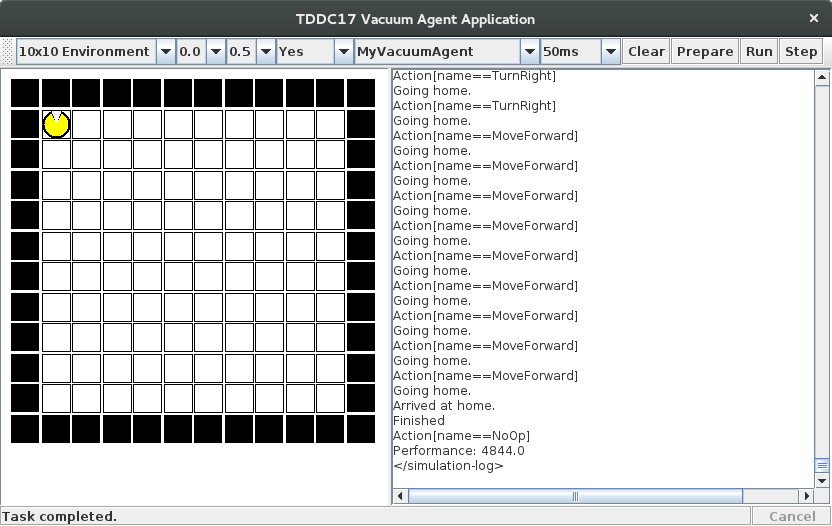
\includegraphics[width=0.83\linewidth]{./images/lab_1.png}
    \caption{Screenshot\label{Vacuum cleaner}}
\end{figure}

\thispagestyle{empty}
